%----------------------------------------------------------------------------
\chapter{Design}
\label{cha:design}
%----------------------------------------------------------------------------

In this chapter I will present the design phase of a new model based testing framework, that tries to take into consideration the conclusions of the investigated available testing tools. This framework is need to be complete regarding the whole MBT process and has to help in all phases of the testing.

First the different testing phases will be discussed separately as at the model based testing process specification (Section \cite{sec:process}). Later I will describe the high level design of the framework and the used technologies.

\begin{enumerate}

\item The first step is the creation of the model. There are many possibility to choose from and we want to have a transition based notation that represents some kind of state machine. State machine notations have different level of expression and come with different amount of features. Generally the more feature a modelling language has, the more hard to generate a good quality test suite from it. That's why we need to find a notation that has a suitable level of expressiveness and it is easy to integrate into a complete testing process.

Earlier we saw that the lowest level of state machine notation is some kind of FSM like notation. However FSMs lacks of many features and a real world software is hard to model with it. Actions, guards, events are not even parts of the improved EFSM notation, so we need to find something more expressive.

Many tools have an UML like notation, but they either can not fully take advantage of the many features of this modelling language or simply avoid their usage. That is not surprising because UML was not designed for testing purposes. UML has just all the features, that are needed to describe the behaviour of a real life software, but some of its feature are hard to utilise during the test generation process. Moreover it lacks some important feature, that a test model has to bear with.

It would be ideal if the test model would express the output of the state machine, because determining the expected output would be trivial by the test generation process. However an UML like semantics and syntax would be easy to adopt by the test engineers, because UML state machines are well known in the industry field and most of its features are easy to use and self-describing. Unfortunately the UML modelling language has lot of implementation and they differ in terms of integrability.

For these issues noted above I think a solution can be the Eclipse Modeling Framework. It is a modelling framework that is built especially for creating tools based on structured models. The EMF platform will be discussed in more details in Section~{sec:softwaredesign}.

EMF models are easy to use, extendable models, that have an UML like syntax.  These models are customisable for the actual needs, and suitable meta-model can be built with the help of the EMF platform. PLCspecif is complete solution that has exactly these previously defined features.

\subsection{PLCspecif}
\label{sub:plcspecif}

PLCspecif is a modelling language intended to be a formal, modular, hierarchical behaviour specification method for describing PLC programs. It was created as part of a doctoral programme by Dániel Darvas of the Budapest University of Technology and Economics (BUTE) and the European Organization for Nuclear Research (CERN).

The abstract syntax of the PLCspecif formalism was designed as an EMF metamodel, therefore the figures are following the original EMF denotation. Here I will describe only the concerned parts of the modelling language as the complete feature set goes far beyond this thesis.

\begin{figure}[htp]
\centering
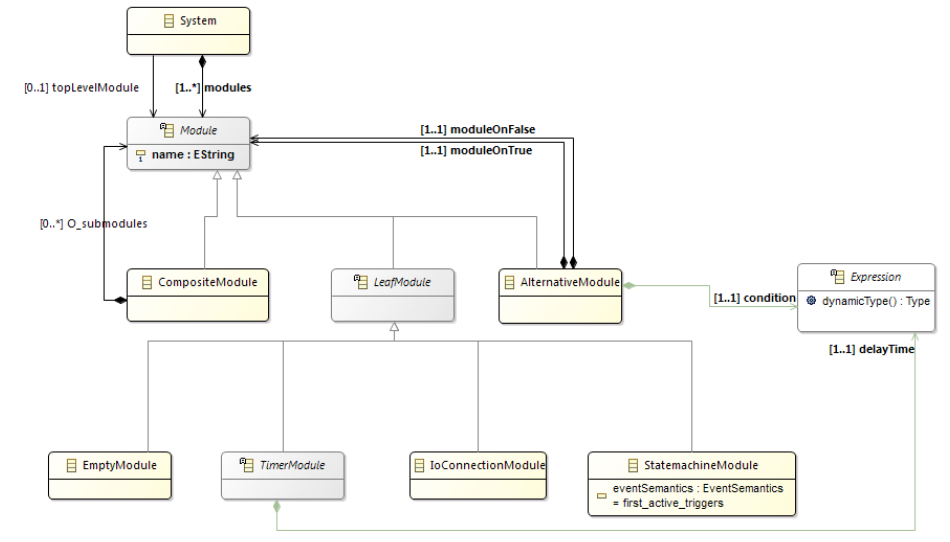
\includegraphics[scale=0.4]{figures/plchsm_modules}
\caption{Module structure of PLCspecif \cite{plcspecif}}
\label{fig:plchsm_modules}
\end{figure}

The specification organised into modules (Figure~\ref{fig:plchsm_modules}), which are either represent a behaviour of concrete module (\texttt{LeafModule}) or they are composite modules containing a set of submodules (\texttt{CompositeModule}).

\texttt{System} is a top-level container that can contain \texttt{modules} from which one module represents the \texttt{topLevelModule}. There are four different module type:

\begin{itemize}
	\item \texttt{StatemachineModule} represents an UML-like state machine.
	\item \texttt{IoConnectionModule} defined by connections between input and output variables.
	\item \texttt{TimerModule} describes a PLC timer in the system.
	\item \texttt{EmptyModule} is a module without any state machine or IO connection.
\end{itemize}

From these module types we are interested especially in the state machine notation. As shown on Figure~\ref{fig:plchsm_statemachine} the metamodel is similar to UML state machine's metamodel described previously (Subsection~\cite{ssub:umlstatemachine}).

\begin{figure}[htp]
\centering
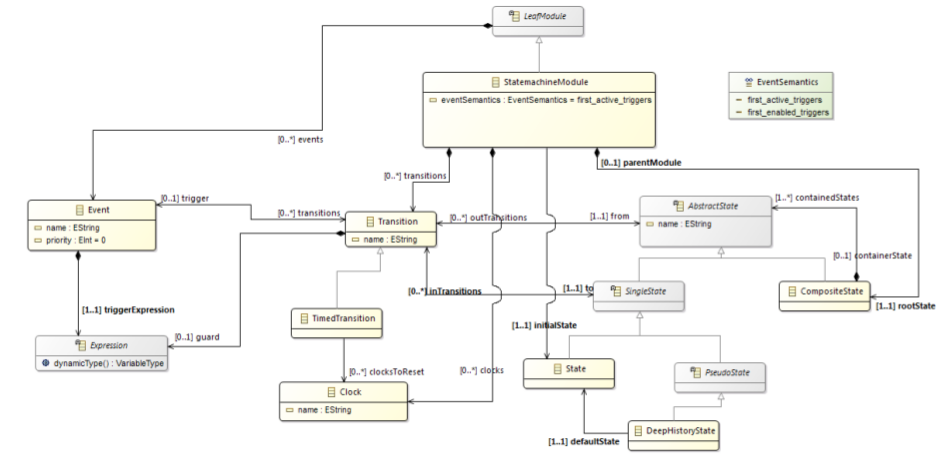
\includegraphics[scale=0.5]{figures/plchsm_statemachine}
\caption{Structure of \texttt{StatemachineModule} \cite{plcspecif}}
\label{fig:plchsm_statemachine}
\end{figure}

On the other hand PLCspecif state machines have some differences from the UML notation:

\begin{itemize}
	\item There is a root state, that recursively contains all of states.
	\item There are pseudo states (\texttt{DeepHistoryState}), which can save a state configuration for its container state.
	\item There are \texttt{TimedTransitions}, which are transitions having time-related conditions.
	\item With \texttt{Clocks} it is possible to define synchronous stopwatches, which can measure the elapsed time since last reset.
	\item Parallel regions are not allowed.
	\item Initial state can not be defined for composite states.
	\item At every moment, exactly one atomic state can be active. 
\end{itemize}

Beside these differences PLCspecif has a bigger difference, which can improve the usability of a test model. Modules can handle input and output variables and can define their outputs using \texttt{VariableDefinitionExpression} objects (Figure~\cite{fig:plchsm_variables}). PLCspecif offers a wide range of possibilities to define an \texttt{Expression}, e.g. \texttt{SwitchCaseTable}, \texttt{DnfExpression}, \texttt{Contant}, \texttt{UnaryOperation}, \texttt{BinaryOperation}, \texttt{NaryOperation}. In our case the output definition of a single state machine can be a switch case table, where conditions checks whether the state machine is in a particular state, and the values are the possible values given by a variable or constant.

\begin{figure}[htp]
\centering
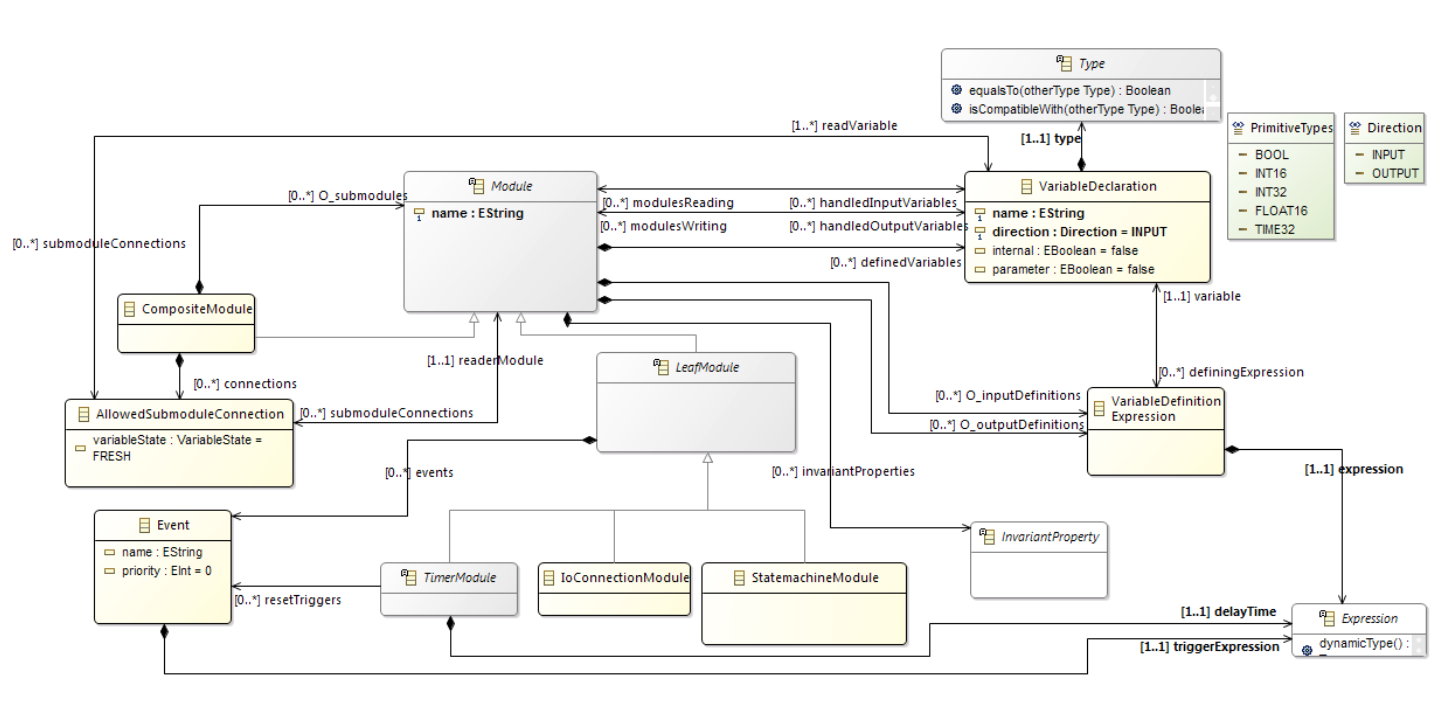
\includegraphics[scale=0.5]{figures/plchsm_variables}
\caption{Variables in PLCspecif \cite{plcspecif}}
\label{fig:plchsm_variables}
\end{figure}

We can see, that PLCspecif has some advantage over traditional UML modelling language in the field of model based testing:

\begin{itemize}
	\item EMF Ecore is a reference implementation of OMG's Essential Meta-Object Facility, that's why syntax should conform with the original UML denotation.
	\item PLCspecif is rather a subset of the UML state machine language, and so it is more simple.
	\item PLCspecif is able to express natively the outputs of a state machine, which can be utilised greatly by the test case generation.
	\item As PLCspecif is based on the EMF Ecore metamodel engineers can take advantage of the entire EMF ecosystem and tooling by the whole MBT process.
	\item UML language has only an informally given semantics, while PLCspecif has a complete formal behaviour specification.
\end{itemize}

% subsection plcspecif (end)

\item The next step of model based testing is the test planning.

The scope of a generated test suite is always is referred to the corresponding state machine. In reality following the Law of Demeter and decoupling, that would mean one class or two classes.

Another important question to discuss is the specification of chosen test selection criteria. We saw at the conclusions of the investigation of related works (Chapter~\cite{cha:relatedwork}), that even the most general and simplest criteria are not fully supported by all the available tools. They either implement complex criteria with a less useful, simple model, or they work with an expressive model and do not support the criteria completely.

At this point I tried to find a golden mean between the different approaches. I chose to implement the basic structural model coverage criteria (full state and transition coverage) on a model with moderate level of expressiveness. Formalisation of this criteria is mostly trivial and left to the implementation chapter (\cite{cha:implementation}).

\item The third step is the test case generation. After examining the available tools we saw, that generally simple test case generation algorithms work fine on simple SUT representations, but as we increase the level of expressiveness so gets also the execution more slower. To generate test suites from complex models we need something more powerful.

Traditional MBT test generation technologies involve model checking, deductive theorem proving and constraint solving. These methods all embed and utilise some powerful mechanism to generate test cases using complex criteria and models. To get the most of these methods usually an intermediate model is used, that maps the original test model to an applicable form and can be executed by e.g. a model checker. That's why our test model should be easily transformable to the intermediate model's notation.

\subsection{Alloy}
\label{sub:alloy}

Alloy is a formal modelling language based on first-order logic to define structures, complex structural constraints and behaviour. Alloy can be utilised with a tool, called Alloy Analyzer to automate the verification process.

The language has been developed on MIT and the first prototype was finished in 1997 in the form of a limited object modelling language. Later the features, performance and scalability have been improved.

Alloy is a declarative language, so that it describes the behaviour without giving the precise execution mechanism. The language was influenced by the Z notation, which is a formal specification language used describing and modelling computer programs and systems. In contrary of Z, Alloy was designed for automatic analysis.

OCL (Object Constraint Language) with UML are often used by MBT tools for expressing SUT behaviour. UML semantics can be imitated by an Alloy model, but Alloy can do even more. As OCL similar to Alloy, but the latter has a more conventional syntax and simpler semantics. So Alloy can combine the features of the two OMG standards and can serve as the input model of a model based testing tool.

Alloy Analyzer transforms problems into SAT formulas to solve them. The solver was inspired by model checkers, but it is implemented as a constraint solver, performing verification within a bounded scope. In constraint programming relations between variables are noted in the form of constraints, that will be solved by giving a value to each variable so that the solution is consistent. If the constraints are inconsistent, then the problem is said to be unsatisfiable.

Alloy version 4 ships in the form of a self-contained JAR file, which includes a variety of supported SAT solver, the standard Alloy library, tutorial examples and an extensive API, that's why it is easy to incorporate into a custom solution.

To summarise the statements above, Alloy has the following benefits:

\begin{itemize}
	\item Alloy are largely compatible with the UML notation. Transforming a model given by any state machine notation should not be a problem.
	\item Alloy is a declarative modelling language, which has the same advantages as any other declarative language. Using a declarative language often results reusable code, and smaller codebase as the imperative versions.
	\item Alloy Analyzer has a convenient API, which are easy to integrate in a tool written in Java.
\end{itemize}

% subsection alloy (end)

\item The last step of the testing process is the test execution. The available MBT tools seems to avoid the support of this step. This is somewhat surprising, because the real theoretical and technical difficulties are solved in the previous steps.

Test scripts, adaptors and oracles can be generated from the prepared test suite and the SUT. EMF code generation facility are a perfect tool to help by this step, as well as by the test case generation.

\end{enumerate}

\section{Software design}
\label{sec:softwaredesign}

Considering the previously described requirements the testing framework should have the following use cases (see on Figure~\cite{fig:designuc}):

\begin{itemize}
	\item model creation / editing
	\item model validation
	\item test suite generation
	\item test suite execution
\end{itemize}

As PLCspecif modelling framework already realised the first two use case, the testing framework can concentrate on the other two use case.

\begin{figure}[htp]
\centering
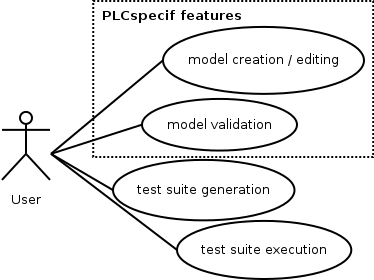
\includegraphics[scale=0.6]{figures/design_uc.png}
\caption{Use case diagram of the testing framework}
\label{fig:designuc}
\end{figure}

Figure~\cite{fig:designcomponents} shows the main components of the testing framework. PLCspecif is based on the EMF platform, but the testing tool can also benefit from the EMF toolset. The required two use case can be realised with two Eclipse plugin. The first plugin will implement the the test suite generation and test execution tooling, the other will be the user interface of the testing tool. Before describing the behaviour and the implementation of the components in depths, the used EMF and the whole Eclipse platform have to be studied.

\subsection{Eclipse Modelling Framework}
\label{sub:emf}

Eclipse is an open source integrated development environment, that contains a base workspace and a highly extensible plugin system. The IDE was written mainly in Java, its primary use is for developing Java, C/C++, PHP applications but there are lot of other supported programming language and framework as well.

\begin{figure}[htp]
\centering
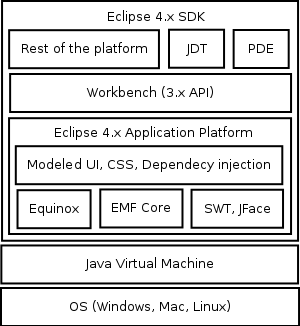
\includegraphics[scale=0.5]{figures/design_eclipse.png}
\caption{Architecture of the Eclipse platform}
\label{fig:designeclipse}
\end{figure}

The required tools for Java development are provided by the Java Development Tools (JDT), see on Figure~\cite{fig:designeclipse}. JDT includes Java editors, refactoring support, debugger, compiler and an incremental builder, that recompiles only those files, which have changed or their dependencies.

Plug-in Development Environment (PDE) provides tooling to extend the capabilities of Eclipse through plugins. Eclipse gained its popularity and power at first from its plugin system. In fact everything is a plugin in Eclipse, except a small run time kernel. All feature are developed and integrated in the same way as a plugin, that's why third party developers are able to join and improve the Eclipse ecosystem.

\begin{figure}[htp]
\centering
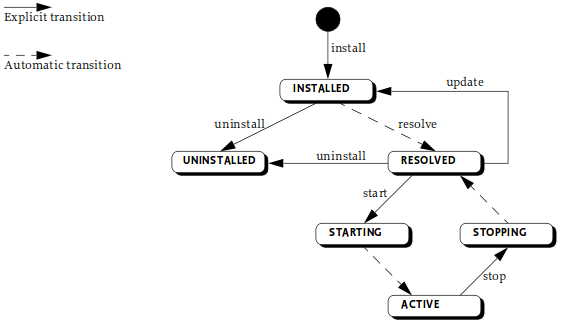
\includegraphics[scale=0.5]{figures/design_osgi.png}
\caption{Lifecycle of OSGi bundles (Eclipse plugins)}
\label{fig:designosgi}
\end{figure}

Plugins are the base elements of the Eclipse component model. These plugins are in reality equal with OSGi bundles. OSGi is a modular system and service platforms, that implements a dynamic component model. The OSGi framework manages the bundles and their class loading, and provides a dynamic, runtime lifecycle management.

OSGi support runtime installation, starting, updating, stopping and uninstallation of the bundles (Figure~\cite{fig:designosgi}). When an application is started, bundles are in installed state. If all dependencies are met, then it changes to resolved state. Once a bundle is resolved, it can be started. Finally it becomes active and is able to interact with other bundles.

Essentially the OSGi bundles are JAR files with a manifest, that describes the dependencies of the bundle. The only difference is between bundles and plugins, that plugins have a \texttt{plugin.xml} file in their root directory, which contains metadata about the plugin. This plugin manifest provides an other way to extend the features of a particular plugin, called extensions and extension points.

\begin{figure}[htp]
\centering
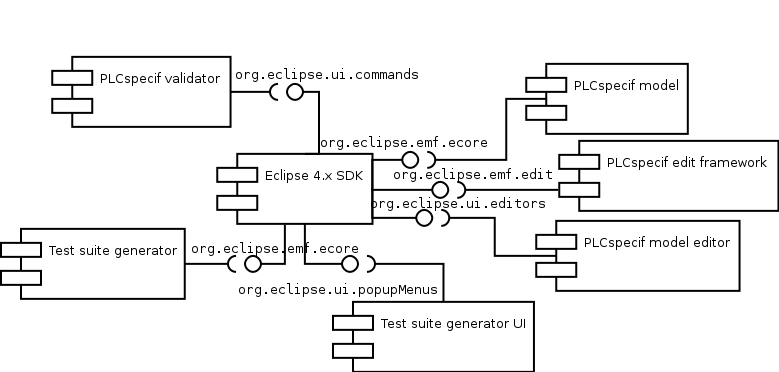
\includegraphics[scale=0.5]{figures/design_components.png}
\caption{Component diagram of the testing framework}
\label{fig:designcomponents}
\end{figure}

Extension points are considered public API, that other developers can use to build their own extension. Figure~\cite{fig:designcomponents} illustrates the components of the testing framework and which extension points they use to communicate with the Eclipse SDK. For example the test suite generator UI uses the \texttt{org.eclipse.ui.popupMenus} extension point to show a new menu item in the generated model editor's context menu.

When Eclipse starts, the platform runtime (Equinox) scans the manifests of the available plugins and builds a plugin registry. These plugins are discovered at the startup, but only activated by the actual usage, this is called \textit{lazy activation}. Lazy activation is enabled by the previously described OSGi platform, which results considerable performance improvements.

Eclipse user interface is built by two other important components of the platform. Eclipse Modeling Framework (EMF) is used to generate a model workbench, that will be rendered into views. Default view renderer uses the Standard Widget Toolkit (SWT) to generate the code of the UI.

EMF is basically a modelling framework and code generation facility for building model based tools. From a created model specification EMF is able to generate model classes, adapters for interacting with the model and a basic model editor.  Models can be specified using annotated Java classes, UML or XMI. XMI (XML Metadata Interchange) is a standard to exchange metadata information and it integrates three OMG standard e.g. UML, XML and MOF (Meta Object Facility, for describing metamodels). EMF consists of three main parts: EMF (Core), EMF.Edit, EMF.Codegen.

EMF is based on a metamodel, called the Ecore metamodel, which can express other models by its components. Ecore is the key to take advantage of the entire EMF ecosystem. Thus Ecore usually used to define a custom metamodel specialised for the actual needs. The core package provides runtime support for models, including change notification, model persistence and an API to manipulate models.

EMF.Edit provides generic reusable classes for building editors for the previously created models.

EMF.Codegen can generate all part of a complete model editor. The first level of code generation is the model generation. This consists of Java interfaces, implementation classes and factories. On second level resides the adapter classes, which adapt the model classes for editing and display. The highest level is the editor, where a basic model editor is generated to start with.

EMF have tools for model transformation as well. There are frameworks, that allows the engineers to use model-to-model and model-to-text transformations. For example ATL supports model-to-model, Acceleo provides ways to transform models into text representations.

% subsection emf (end)

% section softwaredesign (end)

% chapter design (end)